\documentclass{article}
\usepackage[utf8]{inputenc}
\usepackage{amsfonts}
\usepackage{graphicx}
\usepackage{pdfpages}

\graphicspath{ {./figures/} }

\title{Unsupervised Sentiment Analysis}
\author{by RODRIGUES PEREIRA Lucas and PONT Mathieu\\\\directed by FEBRISSY Mickael and LABIOD Lazhar\\\\Paris University, France}
\date{May 2019}

\begin{document}

\maketitle

\abstract{blablabla}



\section{Introduction}

Sentiment Analysis (or opinion mining) is the process of finding the sentiment of a document (text, audio etc.). In the simpler form the sentiment found is rather positive, negative or neutral, but it can be more complex like a rating (from 1 to 5 with 1 being the most negative and 5 the most positive, for example).

Unsupervised learning (or clustering) is the process of partitioning a dataset in different groups having similarities, without the help of an oracle (a "teacher" saying the answer, i.e. the real group of each data).

During our computer science master degree at Paris University we were asked
to do sentiment analysis on the "Scale Movie Review Dataset" (Bo Pang et al. [2005]) using unsupervised learning. This dataset is composed of 5006 movie reviews from 4 different authors. Each review has already it's own label but the goal of this work is to see what can do unsupervised learning on this kind of problem. The label is a rating like described upper (1 to 5 stars).



\section{Related Work}



\section{Preprocessing documents}

Some preprocessing are needed to correctly use the documents for sentiment analysis. The more different words we have, the more difficult it will be to classify them. Therefore we want to remove words that are not important for the classification task. 

We search words that doesn't have any semantic values like the word \textit{"the"} or \textit{"you"} for example, we call this kind of words \textit{stop words}. We can also remove punctuation, numbers and put each word in lower case. Another preprocessing called \textit{lemmatization} tries to change each word into it's word stem. For example the word \textit{"gone"} will become \textit{"go"}. We have removed the words that appears less than 10 times across all the documents, indeed if a word is very rare then it's probably not important.

The python library \textit{nltk} gives us a lot of tools to do this kind of preprocessing. After these preprocessings we finally had 9749 different words in total.



\section{Encoding documents in vector format}

The first step to do sentiment analysis is to encode all documents in a vector format that will be used as input for a classification algorithm for example. 

One of the simplest encoding is the \textit{bag of words}, it's simply an histogram of the words present in each document. The output is a matrix \textbf{X} $\in \mathbb{R}^{n \times d}_{+}$ where \textit{n} is the number of documents and \textit{d} the total number of words within all documents. $x_{ij}$ is the number of times the word corresponding to the column \textit{j} appears in the document \textit{i}.

Another method, based on the \textit{bag of words}, is the \textit{TF-IDF score} that stands for \textit{Term Frequency and Inverse Document Frequency}. This score is computed for each word in each document. It gives us in output a matrix \textbf{X} with the same properties than with the \textit{bag of words} except that we multiply the frequency of the word in the document by a factor depending on the frequency of the word across all the documents like in equation \ref{eq:tf-idf}. 

\begin{equation} \label{eq:tf-idf}
x_{ij} = tf_{ij} \times \log\frac{N}{df_{j}}
\end{equation}

Where $tf_{ij}$ is the frequency of word \textit{j} in document \textit{i}. \textit{N} the total number of documents. $df_{j}$ is the number of documents containing the word \textit{j}. Multiplying the second factor to the frequency of the word allows us to give more importance to word that are rare across all documents. Indeed words that occurs frequently across documents will not help us very much to discriminate them.

Finally we can apply L2 normalization to make each vector unit length, i.e. its norm equals 1. 

For our first experiments we used the \textit{TF-IDF} matrix with L2 normalization.

There are other ways to represent a document in vector. One of them is Doc2vec based on Word2vec


\section{Sentiment analysis experiments}

Here we use many unsupervised algorithms trying to find the correct class of each document.


\subsection{K-Means and Spherical K-Means}

The idea of these algorithms is to create \textit{k} clusters. Each of them gather documents by their similarities measured by a distance. K-Means uses Euclidean distance while Spherical K-Means uses cosinus distance.

The main difference is that Euclidean distance will regroup data points having similar coordinates whereas cosinus distance will regroup data points having their vector pointing in the same direction.

\paragraph{Elbow criterion.}
To find the value of \textit{k} we can use the elbow criterion. It implies to compute the algorithm for many values of \textit{k} and measure the percentage of variance explained by the clusters. For each \textit{k} we need to run the algorithm many times because the result depends on the initialization of the clusters which changes for each execution.

For a certain \textit{k} adding another cluster will not really help us in the data modeling, it will not add much to the variance explained. The behaviour expected is to see the first clusters adding a lot to the variance explained then the gain for each cluster added will drop and ideally we should see an angle in the graph.

\begin{figure}[h] \label{fig:elbow}
\centering
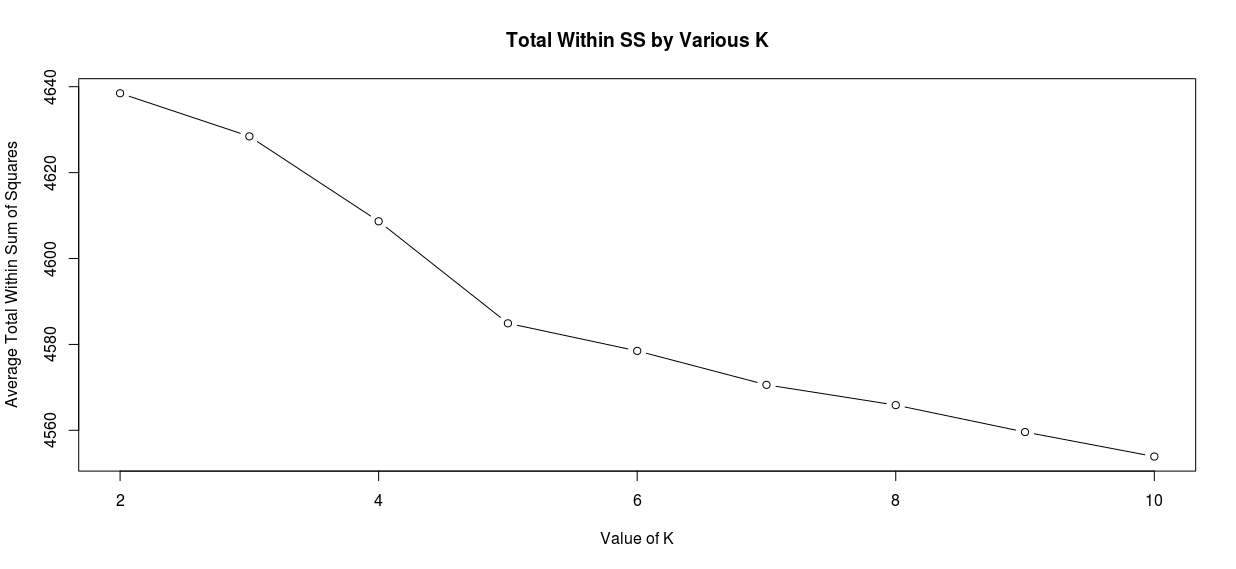
\includegraphics[width=\textwidth]{Kmeans_tf-idf-l2_elbow_criterion.png}
\caption{Elbow criterion for K-Means algorithm.}
\end{figure}

We can see in figure \ref{fig:elbow} the elbow criterion for K-Means with the total within sum of squares as a measure. We can easily see an angle in the curve for the value \textit{k = 5}. This make sense because our documents are separated in 5 classes.

\paragraph{Documents clustering.}
Then we use the K-Means and Spherical K-Means to separate our documents in clusters.

\begin{figure}[h] \label{fig:kmeans}
\centering
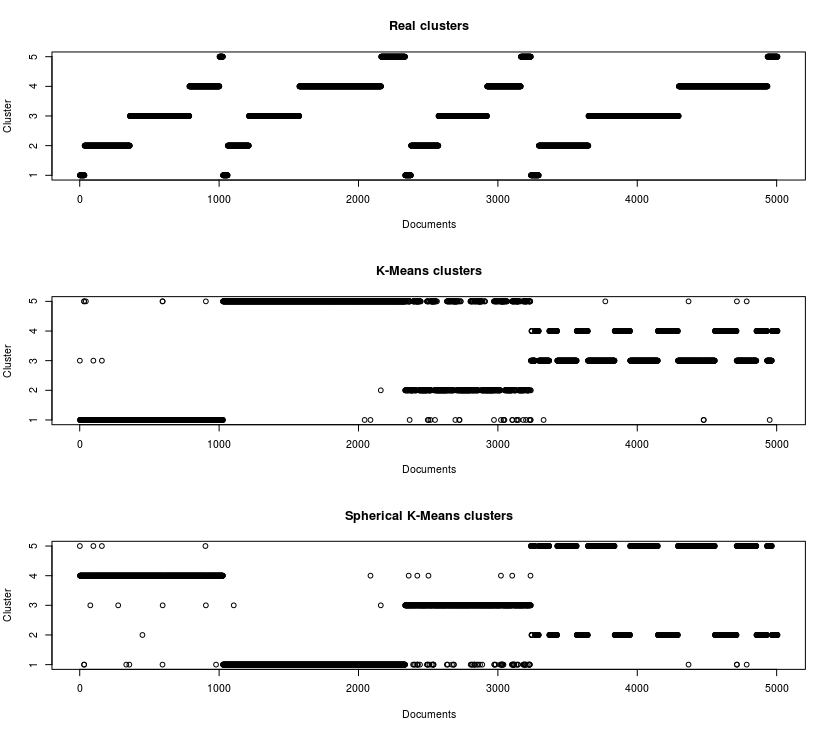
\includegraphics[width=\textwidth]{kmeans_and_skmeans.png}
\caption{Cluster of each document with K-Means.}
\end{figure}

\subsection{Non-Negative Matrix Tri-Factorization (NMTF)}

\paragraph{SentiWordNet}
This dictionary is composed of a lot of words (more than 150 000) and each of them is associated with two scores

SentiWordNet founds 78\% (7604 in 9749) of the vocabulary of our documents.

\subsection{Autoencoder}



\section{References}
Bo Pang and Lillian Lee. 2005. Seeing stars: Exploiting class relationships for sentiment categorization with respect to rating scales.

\end{document}

